\chapter{Event Detection System Using Compressive Sensing}
\index{Event Detection System Using Compressive Sensing@\emph{Event Detection System Using Compressive Sensing}}
\label{chp:event-det}

In this chapter, we show how compressive sensing technique can be applied to build an event detection system in a major cellular network using customer care call data. 

\section{Problem Formulation}
\label{sec:problem-formulation}

\para{Background:} This study uses data derived from operational
records of calls to customer support centers of a major mobile service
provider. We now outline how these records are generated at the
service center, and then describe a subset of the records that are
used for this study. 

When a customer calls the customer support,
the call will first reach an Interactive Voice Response (IVR)
system, an automated system configured with
pre-defined menu. Based on the selected menu, the customer's call
is either self-served
or routed to one of the customer care call centers to be answered by an agent.
Work force management for customer call centers are often performed
according to the type of plan the customer has (\eg, business or
consumer, referred as ``work group'') and what type
of issues the customer has (\eg, device, billing, performance
issues). 

Upon handling each customer care call, the call agent will
open a case in the ticketing system, and
% if this is a new issue which has not been reported by the customer
% before. The call agent will 
label the case using a ``three-level pre-defined categories'' to indicate
the customer's issue or need. 
Detailed notes are also input into
the system based on the conversation with the customer. After the
customer's need is satisfied and case is resolved, a ``call resolution'' code
is also entered into the system.  
% Although customers are uniquely distinguished by means of
% hashed anonymized identifier in the records created at calling time,
% neither this nor the detailed notes were included as data for our study. 
Although the detailed notes may provide more detailed information and
help detect anomalies, 
they are used in this study due to the privacy
issues and the challenge of using natural language to process them.
Therefore, this chapter focuses on using pre-defined categories of the calls to
detect anomalies. 


\iffalse
\para{Background:} An incoming customer's call
% by dialing the toll free number,
first reaches an Interactive Voice Response (IVR)
system, an automated system configured with
a pre-defined menu. Based on the selected menu, the customer's call
is either self-served
% (e.g., checking account balancing)
or routed to one of the customer care call centers to be answered by an agent.
Work force management for customer call canters are performed
based on the type of plan the customer has (\eg, business or
consumer, referred as ``work group'') and what type
of issues the customer has (\eg, device, billing, performance
issues). Upon handling each customer care call, the call agent will
first open a case in the ticketing system, % if this is a new issue which
% has not been reported by the customer before. The call agent will
and label the case using a three-level pre-defined categories to indicate
the customer's issues or need. 
% what issues the customer has or what need the customer asks for (we
% refer them as ``customer need''). 
Detailed notes are also input into
the system based on the conversation with the customer. After the
customer's need is satisfied and case is resolved, a call resolution code
% (we refer it as ``call resolution'')
is also tagged into the system. % according to how the case is resolved.

Our study uses the records that call agents input into their
ticketing system. There is a unique record (identified by ticket
number) corresponding to each customer care calls that handled by call
agents. Each record contains timestamps of the start
and the end of the customer care call, work group, three levels of
customer need, call resolution, and highly coarse grained geographical
location of the customer.
\fi

\para{Customer care calls dataset:}
The data set for this study is derived from several million calls
received at the service centers in 5 months during 2011.
Each record in the dataset comprises the following subset of
information related
to a call: {\em work group}, {\em call resolution} (as described
above) 
and the category ascribed to the call, comprising three levels 
customer need: {\em customer need level 1}, {\em customer 
need level 2}, and 
{\em customer need level 3}.


\iffalse
 that as the categories of the call. 
We collected over 3 millions calls from 2011 August to November from the
mobility service customer care centers in a major network service provider. 
A record is generated from each of such call and takes 
{\em work group}, {\em call resolution} 
and {\em customer need level 1}, {\em customer 
need level 2}, and 
{\em customer need level 3} as the categories of the call. 
{\em work group} indicates 
the working group which is supposed handle the call issue. {\em call 
resolution} indicates how the call issue is resolved. {\em customer need level 1}, 
{\em customer need level 2}, and 
{\em customer need level 3} are pre-defined classes labeled to each 
call by customer care representatives. 
\fi

There are 141 work groups, 5394 call resolutions, 170 level-1
categories, 765 level-2 categories, and 2882 level-3 categories. 
Data do not contain any information concerning calls that did
not progress beyond the IVR system. 
Figure~\ref{fig:category_distribution} shows the normalized call distribution in the most popular 10 categories 
among {\em work group}, {\em call resolution} and 3 levels of {\em customer need}. We can observe that the 
top 10 categories account for 30-70\% of calls. Moreover, top 10\% categories account for 75-90\% of calls. 
In spite of the significant amount of calls in top 10\% categories, we cannot simply use these categories for 
anomaly detection because there are many anomalies dominated by the remaining 90\% categories. 
For examples, ``Technical'' is a level-1 category which does not belong to the top 10\% categories but
it is one of the dominant factors in 73\% of outage events observed from our dataset. 
% 19 out of 26 outage events
% Table \ref{table:top-work-res} and \ref{table:top-lv1-3} show 
% the most popular 10 categories among {\em work group}, {\em call resolution} and 3 levels
% of {\em customer need}. 
\comment { % XXX: should we remove it to avoid confusion?
We can observe two things from the table. First, top 10\% categories account for 75\%-90\% of calls.
Second, some categories have similar name. For example, in Table~\ref{table:top-lv1-3}, 
``Plan'' and ``Plans and Features'' are two different categories in customer need Level 1
but have similar name. It can confuse customer care representatives when they label a call.     
}


\begin{figure*}
\centering
\subfigure[Work Group (141 categories)]{\includegraphics[width=\figurewidthE]{./Figs/category_dist_workgroup.eps}}
\subfigure[Call Resolution (5394 categories)]{\includegraphics[width=\figurewidthE]{./Figs/category_dist_resolution.eps}}


\subfigure[Level-1 (170 categories)]{\includegraphics[width=\figurewidthE]{./Figs/category_dist_lv1.eps}}
\subfigure[Level-2 (765 categories)]{\includegraphics[width=\figurewidthE]{./Figs/category_dist_lv2.eps}}
\subfigure[Level-3 (2882 categories)]{\includegraphics[width=\figurewidthE]{./Figs/category_dist_lv3.eps}}
\caption{The normalized number of calls.}
% \caption{The normalized number of calls in the most popular 10 categories 
% among {\em work group}, {\em call resolution} and 3 levels of {\em customer need}.}
\label{fig:category_distribution}
\end{figure*}


\comment{ %imc-cut
\begin{table}
\centering
\begin{tabular}{|l|c|}
\hline
type of category & \# of predefined classes \\ \hline
work group & 230 \\ \hline
call resolution & 5394 \\ \hline
customer need level 1 & 170 \\ \hline
customer need level 2 & 765 \\ \hline
customer need level 3 & 2882 \\ \hline
\end{tabular}
\caption{Number of predefined classes for each type of category}
\label{tab:categories}
\end{table}
}


\para{Real anomalies:}
In addition, we get ground truth from National Call Center Operations 
(NCCO) reports, in which anomalies are marked manually by monitoring 
the patterns of customer calls, activity of the IVR system, and network traffic. This process is
extremely time-consuming and vulnerable to human errors, which
motivates us to develop an automatic anomaly detector.

Table~\ref{tab:ncco-report} shows an example of NCCO report.
Each anomaly in NCCO reports contains the following information: 
an {\em event status} indicates the anomaly is first reported ({\em initial}),
{\em updated}, or {\em resolved}; a {\em business unit} and {\em primary system} indicate which aspect of system
is impacted by the anomaly; and a {\em region} indicates the impacted region.
A {\em start time} labels the time when the anomaly is observed, and
{\em resolved time} labels the time when the support team reports
that the anomaly has been resolved. In this example, the anomaly is just reported,
so the {\em resolved time} is unknown. There is also a description of the
anomaly, \eg, outage events or performance  degradation. 
We designated the {\em start time} as the time at which an anomaly
is detected. There could be a gap between the time that anomalies are observed 
in NCCO report and perceived by customers.

% XXX: why our method has low recall
Since our approach uses only customer calls data to detect anomalies
while the ground truth from NCCO reports is derived based on the more
complete information (\eg, activity of the IVR system and network traffic), 
we do not expect our approach can detect all anomalies.

\begin{table}
\centering
\begin{tabular}{|l|}
\hline
\textbf{Event Status}: Initial \\
\textbf{Business Unit(s)}: Mobility \\
\textbf{Primary System}: Mobility: GSM Voice Networks    \\     
\textbf{Region}: North East \\
\textbf{Start Time}: month day year - time  \\
\textbf{Resolved Time}: Unknown  \\
\textbf{Issue Description}: Boston customers may experience no service or \\
degraded service in the coverage area of the cell sites affected. \\ 
\hline
\end{tabular}
%\vspace*{-0.15in}
\caption{An example of NCCO report}
\label{tab:ncco-report}
\end{table}

\para{Issues:} The call records give us information about
calls in different categories with different metrics. Each category/metric
gives us one timeseries. Our goal is to automatically detect anomalies or
events using all the timeseries. A natural approach is to detect
sudden changes in one or more timeseries. But finding an appropriate
aggregation of the timeseries for accurate anomaly detection is challenging.

\comment{ %% add another example and rephrase
Simply aggregating all of them does not work well. For example, 
% there are 3 major events: one is {\em iPhone4 new announcement} at June 7
% 2010, one is the {\em start of iPhone4 pre-order} at June 15 2010, and
% the final one is {\em iPhone4 releas} at June 24 2010. 
there were 3 major events related to a release of new devices:
{\em new device announcement},
% on June 7 2010,
{\em new device pre-order},
% on June 15 2010,
and {\em new device available}. 
%on June 24 2010. 
As shown in
Figure \ref{fig:cal-volume-timeseries-day}, 
% if we only
% count the calls that are related to ``iPhone'', we can see clearly
% there are 3 spikes related to the above events during the weeks 6, 7, and 8, respectively.. However, if we ony
% monitor the total call volume, we cannot detect the
% events, because the total volume does not change significantly.
if we consider all the customer care calls that are related to 
a new device, we can see clearly there are 3 spikes in the call volume corresponding 
to the above events. However, the events have little impact on the
total call volume, and are difficult to detect using the total call volume.
}
Simply aggregating all of them does not work well. 
Figure \ref{fig:cal-volume-timeseries-day} show two examples.
In the first example, there were 3 major events related to a release of new devices:
{\em new device announcement},
% on June 7 2010,
{\em new device pre-order},
% on June 15 2010,
and {\em new device available}. 
%on June 24 2010. 
If we consider all the customer care calls that are related to 
a new device, we can see clearly there are 3 spikes in the call volume corresponding 
to the above events. However, the events have little impact on the
total call volume, and are difficult to detect using the total call volume.
In the second example, 3G network outage occurred in South Florida on the second day of the third week.
The anomaly can be detected using the weighted sum of call volume from categories
``Technical'', ``Cannot Make or Receive Calls'', ``Voice'', and
``FLP'' (Florida/Puerto Rico area), but not from 
the total call volume.
% increase of event-related calls is much smaller than the total call
% volume. The other reason is
% Moreover, the capacity limit of call centers places an upperbound on
% the number of serviced calls and limits the change in the total volume
Simply aggregating all calls is insufficient because (i) some events only have
impact on a subset of customers and do not lead to significant changes
in total volume, and (ii) even for the events that may potentially
affect the total volume, the capacity of call centers limits the
increase in total volume and makes it difficult to detect. Ideally in this case, we want to detect
events before the capacity limit is reached so that we can increase
call center capacity temporarily in response to the increased demand.


\begin{figure}
\centering
\subfigure[The three vertical lines indicate the time of 3 major events related to Device-A.]{\includegraphics[width=\figurewidthB]{Figs/call_volume_day-norm2.ps}}
\subfigure[An anomaly detected using the weighted sum of several categories]{\includegraphics[width=\figurewidthB]{Figs/anomaly_ex_florida.ps}}
\caption{The total call volume is insufficient to detect events.}
\label{fig:cal-volume-timeseries-day}
\end{figure}


% \subsection{Existing approaches}
% \label{ssec:existing-approaches}
% There are several existing anomaly detection schemes. 
% Holt-Winters algorithm (denoted as {\em HW}) builds a seasonal model for call volume time series 
% using past observations and make forecasts. It detects 
% anomalies by comparing the difference and ratio of the predicted value to actual 
% value. 
% Subspace scheme \ref{Lakhina_sig04} decomposes data into normal and abnormal 
% subspaces using PCA. It include 3 steps: (1) Apply PCA to the testing dataset and examine the 
% projection of testing dataset on each principal axis in order. (2) As soon 
% as a projection is found to exceed a threshold (\eg, 2x standard deviation 
% from mean), the principal axis and all subsequent axes are assigned to 
% anomalous subspace. (3) Detect spikes in the time series projected onto the
% anomalous subspace. 

% To show how these existing schemes perform, we compare the precision and recall using
% HW and Subspace schemes with our proposed scheme (denoted as {\em CS}, will explain the detail in Section 
% \ref{sec:approach}) and a random algorithm which report an anomaly with 0.3 probability
% (shown in Figure \ref{fig:existing_schemes}). 
% {\em HW} has low recall which matches what we observe in Section \ref{ssec:case-study} 
% that only monitoring call volume may miss some anomalies. On the other hand,
% {\em PCA} explores the data projection to each principle 
% component and have higher recall. However, because {\em PCA} is known to be 
% sensitive to outliers, the noisy dataset as customer calls can result in low precision as 
% shown in the figure.

Another natural approach to detect anomalies is to use PCA. For example,
\cite{PCA2} decomposes data into normal and abnormal
subspaces using PCA by (i) applying 
PCA to the testing dataset and examining the projection of testing
dataset on each principal axis in order, (ii) assigning the principal 
axis and all subsequent axes to anomalous
subspace as soon as a projection is
found to exceed a threshold (\eg, 2x standard deviation from mean),
and (iii) detecting spikes in the time series projected onto the
anomalous subspace. We observe its precision (\ie, fraction of predicted 
anomalies that are correct) is not much better than that of a random 
algorithm, which reports an anomaly by tossing a bias
coin of 0.3 (\ie, close to the fraction of time that has
anomalies.) 
% XXX: why PCA doesn't work well in detecting anomalies
\comment {
PCA performs poorly because it looks for
orthogonal axes, but orthogonal axes may not represent the most
important metrics. In addition, PCA is sensitive to outliers, which
can be common in noisy customer call dataset.
}
PCA performs poorly for several reasons. First, large anomalies can 
pollute the normal subspace \cite{PCA-sensitivity} so PCA usually requires 
anomaly-free data for training \cite{PCA-unsupervised}. This could be a problem 
for our dataset because there are average 1.8 anomalies per week in NCCO reports 
and it is hard to find a clean period for training. Second, determining the threshold 
for anomalous subspace is an open question \cite{PCA-sensitivity, PCA-structural, PCA2}. 
Third, PCA is sensitive to noise, which is common in the customer care call dataset. 

In general, the appropriate aggregation depends on the types of
events. Due to a large number of possible types of events and
evolving nature of events, it is infeasible to manually determine the
aggregation for each event type in advance. 
The above results call for a new method to automatically learn the
mapping from the various input metrics to anomalies. The method should
be (i) adaptive to new call labels and events, (ii) highly robust
against noise, which is inherent in call data records due to different
customers' responses to anomalies and inconsistent 
call labelings.



%% =================================================================

\section{Our Approach}
\label{sec:approach}

\subsection{Problem Formulation}

Our main problem can be formulated as follow. We have training and
testing traces, where the training traces contain $N$-dimension input
timeseries and the ground-truth about when anomalies take place and
the testing traces contain new $N$-dimension input timeseries. Our
goal is to determine when anomalies occur in the testing traces. 

We use regression to approach
the problem by casting it as an inference problem of $A x = b$, where
$A(t,i)$ denotes the number of calls of category $i$ at time $t$, $x(i)$ denotes
the weight (importance value) of the $i$-th category, $b(t)$ is an
indicator whether there is an anomaly. We construct $A$ and $b$ from the training traces to solve
for $x$. Then we plug in the estimated $x$ and construct $A$ from
the testing traces to predict $b$ for the testing trace. 
Essentially we view there
exists a linear relationship between the categories values and the
resulting anomalies, and we try to learn the linear coefficients $x$
that automatically combines different metrics to predict the
anomalies. 
As we will show in Section~\ref{sec:evaluate}, a 
simple linear regression model works well, so we believe the 
linear assumption is reasonable.
There are several significant challenges involved in realizing this scheme.

\begin{senumerate}
  \item Dynamic $x$: As the categories and events evolve, the
    relationship between the inputs and the anomalies may also
    change. Therefore $x$ can change over time. 
  \item Under-constraints: The number of categories can be much larger
    than the number of constraints derived from the training traces.
    So we have an under-constrained problem and there are an infinite
    number of solutions. Randomly picking one of them gives an equally
    good fit to the training data, but can give very
    different accuracy for the testing data. Our ultimate
    goal is to find $x$ that can accurately predict the
    anomalies for the testing traces.
  \item Over-fitting: Even if we are fortunate to get long enough
    training traces so that the number of categories is close to or
    smaller than the number of constraints, the weight estimation is
    still challenging because the solution that minimizes the fitting
    error based on the training traces is often not the one that gives
    the closest fit to the testing data. In other words, there can be
    over-fitting issues.
  \item Scalability: There are thousands of categories or dimensions
    and thousands of time intervals. The scalability issue further exacerbates
    when we allow $x$ to change. For example, if there are
    $K$ different $x$'s, the problem size further grows by a factor of $K$.
  \item Varying customer response time: When an anomaly
     occurs, customers respond to it at different time depending on
     the impact of anomaly, the customers' own availability, time of
     day, and day of week. This
     blurs the relationship between $A$ and $b$.
     % fuzzy and not well defined. 
\end{senumerate}    

Below we first develop an approach to address the under-constraints
and over-fitting issues while allowing $x$ to change over time
(Section~\ref{ssec:regression}). Then we reduce the number of unknowns
as well as handle the scalability issues by clustering categories and
identifying important clustered categories (Section~\ref{ssec:scalability}). 
Finally, we use multiple classifiers to enhance the
robustness against noise and different customers' response time (Section~\ref{ssec:aggregation}).


\subsection{Our Regression}
\label{ssec:regression}

%As mentioned in Section~\ref{ssec:important}, we can learn the
%importance value of each category by casting the problem as an
%inference problem of $A x = b$. Different from
%Section~\ref{ssec:important}, which aims to pick the important
%metrics, which is a binary decision, accurate predicting future
%anomalies requires us to achieve higher accuracy in the weight
%estimation. More specifically, we formalize the anomaly detection
%problem as follow. Let $A_d(t,i)$ denote the value of $i$-th category
%from the traces at time $t$ on the $d$-th day, $x_d(i)$ denote the
%weight of $i$-th variable on day $d$, $b_d(t)$ denote whether there is
%an anomaly at time $t$ on the $d$-th day, where 1 means anomaly and 0
%means no anomaly.
%
%A natural goal is to also minimize the fitting error to the training
%data. However fitting error alone is insufficient for several reasons. First,
%when the number of categories is smaller than the number of
%constraints derived from the previous traces, we have an
%under-constrained problem and there are an infinite number of
%solutions. Randomly picking one of them gives an equally good
%fit to the previous training data, but can give very different
%accuracy on the testing data in the future. Our ultimate goal is to
%find $x$ such that we can use it to predict the anomalies based on the
%new $A$ derived from the testing traces. Second, if we are fortunate
%to get long enough training traces so that the number of
%categories is close to or smaller than the number of constraints, the
%weight estimation is still challenging because the solution that
%minimizes the fitting error based on the training traces is often not
%the one that gives the closest fit to the testing data. In other words,
%there can be over-fitting issues. 

To address the first challenge, we generalize our formulation to $A_d
x_d = b_d$, where $d$ denotes $d$-th day, $A_d(t,i)$ denote the value
of $i$-th category from the traces at time $t$ on the $d$-th day,
$x_d(i)$ denote the weight of $i$-th variable on the $d$-th day, $b_d(t)$
denote whether there is an anomaly at time $t$ on the $d$-th day,
where 1 means anomaly and 0 means no anomaly.

To address the under-constraints and over-fitting issues, we cannot 
simply minimize the fitting error to the training data. 
Instead, we also impose additional structures on the solution. First, we expect
the weight values $x_d$ to be stable across consecutive days $d$. Second, 
we expect $x = [x_1 x_2 ... x_d]$ exhibits low-rank structure due to
the temporal stability in $x$ and the small number of dominant factors
that cause the anomalies. 
% we expect $x = [x_1 x_2 ... x_d]$ exhibits low-rank structure.
%, because there tends to be a small number of dominant factors. 
Therefore, we 
try to find $X$, $U$, $V$ that minimize the combined objective:
\begin{equation}
o(X,U,V) = \sum_d f(X) + \alpha\cdot g(X) + \beta\cdot h(X,U,V),
\label{eq:c(X)}
\end{equation}
where $f(X)$ is the fitting error, $g(X)$ captures the degree of
temporal stability, and $h(X,U,V)$ captures the error in approximating
$X$ as a product of two rank $r$ matrices: $U$ and $V$, where $\alpha$ 
and $\beta$ give the relative weights of temporal
stability and low-rank constraints, respectively, and $r$ is
the desired low rank.
% Our evaluation uses $\alpha = 0.01$, $\beta = 0.1$, and $r=100$. 
Next we elaborate on each term and how to select weights.

\para{Fitting error:} The fitting error is expressed as
%\begin{align}
$f(X) = \sum_d \left\|A_d x_d - b_d\right\|_F^2$ 
%\end{align}
where $\|\cdot\|_F$ is the Frobenius norm 
% \comment{ %infocom-cut
% ~\cite{wiki:Frobenius-norm} 
% }
(with $\|Z\|_F = \sqrt{\sum_{ij} Z(i,j)^2 }$ for any matrix $Z$.)

\para{Incorporating temporal stability:}
To capture the temporal stability, we introduce
a temporal transformation matrix $T$ and define a penalty
function as follows:
\begin{equation}
g(X) \defas \left\| M \ast T^T\right\|_F^2,
\end{equation}
where $M = [x_1 x_2 ... x_d]$ merges all the column vectors into a
matrix and $T^T$ is the transpose of $T$. As in \cite{zhang09sensing}, we use a simple temporal
transformation matrix to minimize the change in $x$ between two consecutive days:
$T=Toeplitz(0,1,-1)$, which denotes the Toeplitz matrix 
with central diagonal given by 1, the first upper diagonal given by -1. That is, 
{\scriptsize
\begin{equation}
 T = \left[
  \begin{array}{rrrrrrrr}
        1 & -1 &  0 &  \ldots \\
        0 &  1 & -1 &  \ddots \\
        0 &  0 &  1 & -1 & \ddots \\
        \vdots &  \ddots &  \ddots &  \ddots   \\
  \end{array} \right].
\end{equation}
}
\para{Incorporating low-rank constraints:}
Finally, to capture the low-rank nature of weight matrix, we
introduce a penalty term function
\begin{equation}
h(X,U,V) \defas \left\|M - U\ast V^T\right\|_F^2
\end{equation}
where $M = [x_1 x_2 ... x_d]$, $U$ is a $N \times r$ unknown factor matrix, and $V$ is a
$d \times r$ unknown factor matrix, and $r$ is the desired low
rank.  Minimizing the penalty term ensures $M$ has a good rank-$r$
approximation: $M \approx           
U\ast V^T$.

\para{Selecting parameters:}
To decide the weights $\alpha$ and $\beta$, we use 6-week data as the 
training set to find the best weights (in terms of evaluation metrics 
discussed in Section \ref{sec:evaluate}) as follow.
% and use them in our evaluation. 
% The selecting procedure is as following.
First, 
$\alpha$ and $\beta$ are chosen to make fitting error, temporal stability, 
and low-rank constraint have similar order of magnitude. Second, we
fix $\alpha$, and keep increasing or decreasing $\beta$ by a factor of
10 each time until the performance does not improve. 
$\beta$ is updated as the one that gives the best performance seen so far. Third, similar to the second step, 
but this time we fix $\beta$ and alter $\alpha$. The second and third
steps are repeated until the performance does not improve for the
training traces. It usually takes 5 or fewer iterations. 
Then we apply the selected parameters to the testing
trace for anomaly detection. 

%Note that in theory, we do not require a separate step of identifying important
%metrics with the current step of inferring the weights of all metrics
%as one. However, for efficiency purpose, we separate these two steps in our
%approach because the step of identifying important metric requires
%working with all metrics, which are potentially thousands and $L_1$
%norm minimization is light-weight enough to work with thousands of
%metrics.

% \subsection{Data Preparation}
% \label{ssec:preparation}

%% \subsection{Customer Care Call Data} 

%% When a customer calls the customer support,
%% % by dialing the toll free number,
%% the call will first reach an Interactive Voice Response (IVR)
%% system, an automated system configured with
%% pre-defined menu. By selecting through the menu, the customer's call
%% is either self-served
%% % (e.g., checking account balancing)
%% or routed to one of the customer care call centers to be answered by an agent.
%% Work force management for customer call canters are often done
%% according to the type of plan the customer has (\eg, business or
%% consumer) (we refer it as ``work group'' in the paper) and what type
%% of issues the customer has (\eg, device, billing, performance
%% issues). Upon handling each customer care call, the call agent will
%% first open a case in the ticketing system if this is a new issue which
%% has not been reported by the customer before. The call agent will
%% label the case using a three-level pre-defined categories to indicate
%% what issues the customer has or what need the customer asks for (we
%% refer them as ``customer need''). Detailed notes are also input into
%% the system based on the conversation with the customer. After the
%% customer's need is satisfied and case is resolved, a resolution code
%% (we refer it as ``call resolution'') is also tagged into the system
%% according to how the case is resolved.

%% In our study, we use the records that call agents input into their
%% ticketing system. There is a unique record (identified by ticket
%% number) corresponding to each customer care calls that handled by call
%% agents. Each record contains information on timestamps of the start
%% and the end of the customer care call, work group, three levels of
%% customer need, call resolution, and highly coarse grained geographical
%% location of the customer.  Note that the data do not contain
%% information on the customer care calls that are self-served by IVR
%% system or dropped due to long waiting time.

\subsection{Reducing Categories}
\label{ssec:scalability}

The regression problem described in Section~\ref{ssec:regression} has
thousands of variables for each day alone and the number further increases with the
number of days. This imposes both scalability issue and exacerbates
under-constraint issue. 
\comment { % XXX: should we remove it to avoid confusion?
Since top 10\% categories account for 75\%-90\% of calls, one intuitive way to
reduce the number of categories is to use the top 10\% categories. It does not
work for two reasons. First, there are anomalies dominated by categories that are 
not belong to top 10\% categories. For example, the 3G network outage shown in 
Figure~\ref{fig:cal-volume-timeseries-day} is dominated by categories
``Technical'', ``Cannot Make or Receive Calls'', ``Voice'', and ``FLP'' where 
``Technical'' and ``Voice'' are not one of top 10\% categories. 
% 3G network outage is one of the major events that we don't want to miss. 
Second, when new categories are introduced for new services/products, 
the call volume is relatively small at beginning. 
Although the new services/products tend to have more problems, they may be ignored if 
only top 10\% categories are considered. 
Therefore, it's not enough to just focus on these fewer categories.
In this study, we reduce the number of categories using clustering and identifying important
categories. 
}

\subsubsection{Clustering Categories}
\label{ssec:preparation}

% The pre-defined three levels of customer need categories are very fine
% grained.  For example, there are 170, 765, and 2882 unique categories
% in the three levels of customer needs, respectively. As a result,
% there can be multiple categories related to a single type of
% issue. This could cause some ambiguity in the process of hand labeling
% customer care calls by agents. Hence, it is quite common to have
% inconsistency across call agents and call centers.

% To enhance scalability and minimize the
% impact of ambiguity and inconsistency in detecting events based
% on the customer needs categories, we cluster relevant categories based
% on string similarity of their names. In particular, we treat each category name as a sequence of characters and adopt the Dice's coefficient~\cite{wiki:dice} using bigram model~\cite{wiki:bigram}, which is widely used in statistical natural language processing to measure string similarity. 

To enhance scalability and minimize the
impact of ambiguity and inconsistency in detecting events based on the 
customer needs categories, we need to cluster relevant categories in advance.
It is infeasible to group categories manually because (i) the number of categories 
changes over time. Categories can be added or depreciated because of the emerging 
or ending of services/products; (ii) each customer care center can change the usage 
of categories; and (iii) there are too many categories. 

One natural approach is to cluster categories base on  the similarity
between timeseries. However, the approach does not work. 
% Take ``Plan'' and ``Plan and Features'' mentioned in Section~\ref{sec:problem-formulation} as an example. 
For example, Figure~\ref{fig:category_volume_change} shows timeseries of different categories. 
We can see that the call volume of category ``Plans and Features'' increases significantly 
while that of the other category ``Plan'' decreases on the same day, because the agents are 
asked to switch to use ``Plans and Features'' instead of ``Plan''. 
%% give a more complicate example why grouping by timeseries similarity doesn't work:
% XXX: is this a good example? later we actually group categories by name
Similarly, we can see the call volume of ``Device'' decreases while that of ``Account''
and ``Equipment'' increases. Although these categories represent the same group 
of calls, their timeseries are not similar.

% \begin{figure}
% \centering
% \includegraphics[width=0.4\textwidth]{Figs/top10_ts.ps}
% \vspace{-0.15in}
% \caption{The number of calls labeled as ``Plan'' and ``Plans and Features''. 
% In the second day of the 6th week, call centers use the latter to replace the 
% former.}
% \vspace{-0.15in}
% \label{fig:category_volume_change}
% \end{figure}
\begin{figure}
\centering
\subfigure[The number of calls labeled as ``Plan'' and ``Plans and Features'']{\includegraphics[width=\figurewidthB]{Figs/top10_ts.ps}}
\subfigure[The number of calls labeled as ``Account'', ``Equipment'', and ``Device'' ]{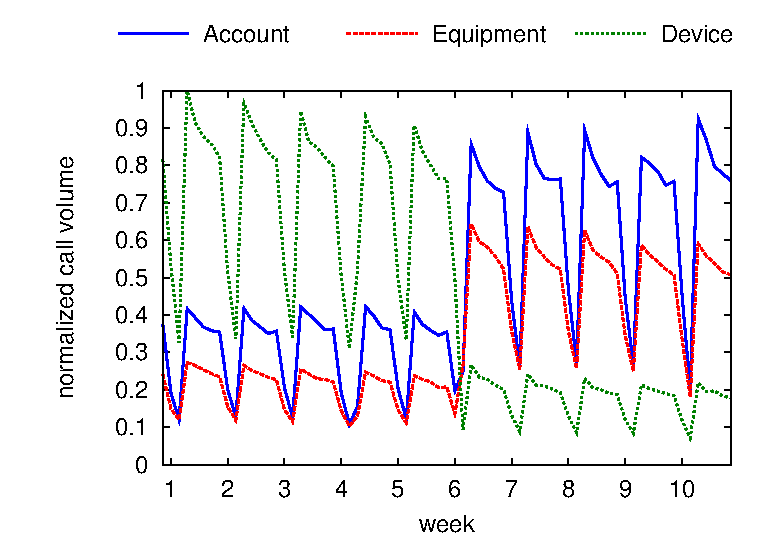
\includegraphics[width=\figurewidthB]{Figs/top10_ts2.ps}}
\caption{Dynamic call labels}
\label{fig:category_volume_change}
\end{figure}

We cluster categories based on the similarity of their textual names
since agents usually classify calls based on the textual names of
categories and different agents may classify similar calls to
different categories with similar texts.
% The clustering method we use is based
% on string similarity of their names.
We treat each category name as a sequence of characters and adopt the Dice's coefficient~\cite{wiki:dice} using bigram model~\cite{wiki:bigram}, which is widely used in statistical natural language processing to measure string similarity. 
The Dice's coefficient $s$ for two string $x$ and $y$ using the bigram model is computed as
$s=\frac{2 \times n_t}{n_x+n_y}$, 
where $n_t$ is the number of character the bigrams in both strings, $n_x$
and $n_y$ are the numbers of big-rams in strings $x$ and $y$,
respectively. The value of $s$ ranges between 0 and 1. A
larger $s$ indicates the two strings are more similar. For example, to
calculate the similarity between strings ``paid'' and ``payment'', we
find the sets of the bigrams as (``pa'', ``ai'', ``id'') and
(``pa'', ``ay'', ``ym'', ``me'', ``en'', ``nt''). These sets have 3 and
6 elements, while only 1 element is common. So we have $s=(2
\times 1)/(3 + 6)=0.22$. By using a threshold of 0.3 for $s$, 
we cluster the customer categories into $96$
at the first level, $354$ at the second level, and $1165$
at the third level. Our evaluate uses these newly computed categories.

\subsubsection{Identifying Important Categories}
\label{ssec:important}

Even after clustering, there are still a large number of clustered
categories. We use the following three schemes to identify important
categories. 

% So we identify important categories by casting this problem
% as an inference problem, and use the following three schemes to solve it.

% We reduce the number of factors by casting the problem
% into an inference problem.In particular, we used and evaluated the 
% following three methods.

\para{Principal component analysis (PCA):} 
% PCA converts a set of
% possibly correlated variables into linearly uncorrelated variables,
% which are called principal components. 
PCA can also be used to identify important categories because
it reduces dimensionality of a multivariate dataset by converting
possibly correlated variables into linearly uncorrelated variables, 
which are called principal components.
% PCA can be performed using
% singular value decomposition of matrix $A$, usually after mean
% centering. 
% XXX: why PCA doesn't work well in identifying important factors
However, using PCA in this context has the same problem as it is used for anomaly detection 
mentioned in Section~\ref{sec:problem-formulation}. As a result,
% The disadvantage of PCA in our context is that 
principal components may not identify the most important categories for 
anomaly detection. For example, 
the 3G network outage event shown in Figure~\ref{fig:cal-volume-timeseries-day}
is dominated by categories ``Technical'', ``Cannot Make or Receive Calls'', ``Voice'', and ``FLP''.
However, the PCA results show that in the top 10\% principal components,
the coefficients of ``Cannot Make or Receive Calls'' and ``Voice'' are small, which
indicates they are not considered as important categories in PCA.


\para{$L_2$ norm minimization:} Another way of finding important
categories is to cast it as an inference problem $A x = b$, where
$A(t,i)$ denotes the value of category $i$ at time $t$, $x(i)$ denotes
the weight (importance value) of the $i$-th category, $b(t)$ is an
indicator whether there is an anomaly. Different from
Section~\ref{ssec:regression}, here we just need to filter out
unimportant categories instead of determining the precise weights. So
here we assume $x$ is constant over time to have fewer unknowns. 

% where $A(t,i)$ denotes the value of category $i$ at time $t$, $x(i)$
% denotes the weight (importance value) of the $i$-th category, $b(t)$
% is an indicator whether there is an anomaly. Essentially we view there
% exists a linear relationship between the categories values and the
% resulting anomalies, and we try to learn the linear coefficients $x$
% that automatically combine different metrics to explain the anomalies.

We obtain $A$ and $b$ learned from
the previous traces. Then we estimate $x$ to best fit the relationship. A
common metric for the best fit is {\em $L_2$ norm minimization},
defined as follows:
%$x$
%which corresponds to (\ref{eqn:reg}) with $J(x) = \|x\|_2^2$.
% $J(\bx) = \|\bx\|_2^2$.
\begin{equation}
% \min_\bx \|{\by} - A {\bx}\|_2^2 + \lambda^2 \|{\bx}\|_2^2.
\min_x \|{b} - A {x}\|_2^2 + \lambda^2 \|{x}\|_2^2,
\label{eqn:L2:0}
\end{equation}
where $\|{x}\|_2 = \sqrt{\sum_{k=1..n} \|x_k\|^2}$.
It can be efficiently
solved using a standard solver for linear least-squares problems.
Then we filter out the categories whose weight $x$ is within a
threshold, which is set to 0 in our evaluation.

\para{$L_1$ norm minimization:} Another approach 
is to use
% (\ref{eqn:y=Ax}) is
{\em $L_1$ norm minimization}, defined as follow: 
% (\ref{eqn:reg}) with 
% $J(\bx) = \|\bx\|_1$ 
%$J(x) = \|x\|_1$ 
% (\ie, the $L_1$ norm of $\bx$).
%(\ie, the $L_1$ norm of $x$).
\begin{equation}
% \min_\bx \|{\by} - A {\bx}\|_2^2 + \lambda^2 \|{\bx}\|_1.
\min_x \|{b} - A {x}\|_2^2 + \lambda^2 \|{x}\|_1.
\label{eqn:L1:0}
\end{equation}
where $\|{x}\|_1 = \sum_{k=1..n} \|x_k\|$. 
$L_1$ norm minimization is often used in situations where 
% $\bx$ 
$x$ 
is
{\em sparse}, \ie, $x$ has only very few large elements and the
other elements are all close to $0$. This is well suited to our goal
of identifying a small number of important factors. As shown
in~\cite{donoho-L1-1}, the minimal $L_1$ norm solution often coincides
with the sparsest solution for under-determined linear systems. As we
will show in Section~\ref{sec:evaluate}, $L_1$ norm minimization performs
the best since it explicitly maximizes sparsity. As before, we filter out the categories whose weight $x$ is within a
threshold, which is set to 0 in our evaluation. 


\subsection{Combining Multiple Classifiers}
\label{ssec:aggregation}

\para{Need for multiple classifiers:} 
Another important problem is what time scale we should use for anomaly
detection. Ideally, we would like to capture all calls triggered
by the same anomaly when learning the weight of the metrics. That is,
$A$ should include the characteristics of all calls corresponding to
that anomaly. However, customers do not respond to an anomaly
immediately and sometimes their response time may differ by hours. But
simply using a large time window is not a good option since we can no longer
detect anomalies in a fine time granularity. 

To address both issues, we use a reasonably small bin size: 1 hour, but include
calls made in previous $n$ and next $m$ hours as additional
features. That is, we use $A_d(t-m,t-(m-1),...,t-1,t,t+1,...,t+n)$, which denotes the values of 
$N$ categories in the traces from time $t-m$ to time $t+n$. 
So there are altogether $(m+n+1) \times N$ features and $x_d$ also now
has $(m+n+1) \times N$ elements, which are the weights of all these
features. $b_d(t)$ remains the same as before (\ie, whether there is
an anomaly at time $t$).

However it is challenging to select $m$ and $n$ a priori. One set of
values may work well on some data but not on others. % The main
% reason is that human respond to anomalies in different ways depending
% on the impact of anomalies, their own availability, and time of
% day.
Therefore we use multiple classifiers, where each classifier uses
one set of $m$ and $n$, and then we aggregate the results of all the
classifiers. The intuition is that it is more likely to be a real
anomaly if lots of classifiers claim so.

\para{Aggregating multiple classifiers:} 
We apply each classifier independently to the testing data and 
returns a binary timeseries $pb(c, t)$. $pb(c, t)=1$ denotes that there 
is an anomaly detected by classifier $c$ at time $t$. $pb(c, t)=0$ 
denotes there is no anomaly detected. We aggregate $pb(c, t)$ by assigning 
a weight $w_c$ to each classifier. We detect an anomaly when $\sum_{c} w_c pb(c, t) 
> threshold$. Our evaluation uses a threshold of 0.3.

We calculate $w_c$ for a classifier $c$ by applying 2-fold 
cross-validation to the training data.
The 2-fold cross-validation partitions the training data into two parts. In 
the first round, it uses the first partition for training and the second partition for 
testing. Since we know the ground truth in all training data, we can evaluate 
how the classifier performs in cross-validation by calculating the accuracy
(\ie, the fraction of correct prediction) in the second partition. Similarly, 
in the second round, we use the second partition of the training data for training, 
use the first partition for testing, and calculate the accuracy in the first partition.
Therefore, with the 2-fold cross-validation we can get an average accuracy $a_c$ in 
training set which gives us an estimate how the classifier may perform.
Then the weight of each classifier is assigned as the normalized 
accuracy: $w_c = a_c / \sum_{c} a_c$.

%% =================================================================


\section{Evaluation}
\label{sec:evaluate}

%\subsection{Evaluation Methodology}

%We evaluate our methods by altering one component at time to see how it impacts 
% the final results.

\begin{figure*}[ht]
    % \centering
    \begin{minipage}{\figurewidthE}%
        \centering
        % \includegraphics[scale=0.5]{Figs/identify.eps}
        \includegraphics[width=\figurewidthE]{Figs/identify.eps}
        \caption{\small{Varying schemes for features.}}
        \label{fig:identify}
    \end{minipage}
    \begin{minipage}{\figurewidthE}%
        \centering
        % \includegraphics[scale=0.5]{Figs/regression.eps}
        \includegraphics[width=\figurewidthE]{Figs/regression.eps}
        \caption{Varying regression methods.}
        \label{fig:regression}
    \end{minipage}
    \begin{minipage}{\figurewidthE}%
        \centering
        % \includegraphics[scale=0.5]{Figs/multi-num-classifier.eps}
        \includegraphics[width=\figurewidthE]{Figs/multi-num-classifier.eps}
        \caption{Varying the number of classifiers.}
        \label{fig:multi-num-classifier}
    \end{minipage}
\end{figure*}


We use the following metrics to quantify the accuracy:
\begin{align}
&recall = \frac{tp}{tp+fn}\\
&precision = \frac{tp}{tp+fp}
\label{eqn:metric}
\end{align}
% \begin{equation}
% accuracy = \frac{tp+tn}{tp+tn+fp+fn}
% \label{eqn:accuracy}
% \end{equation}
where $tp$ is the number of true positives (\ie, correctly detected anomalies),
$fp$ is the number of false positives (\ie, incorrectly detected anomalies),
% $tn$ which denotes $true negative$ are the correct obsense of anomalies, 
and $fn$ is the number of false negatives (\ie, missed anomalies).
In addition, we integrate precision and recall into a single metric
called {\em F-score}~\cite{wiki:F-score}, which is the harmonic mean
of precision and recall: {\em F-score} $ = \frac{2}{1/precision +               
1/recall}$. For all three metrics, larger values indicate higher accuracy.
Unless otherwise specified, we use 30 classifiers.

%\subsection{Performance Results}

% use the best regression and try L1, L2, random, textual based
% etc. to show L1 is the best

\para{Identification of important features:} We first evaluate how 
different feature selection algorithms impact 
the performance. We vary the methods of identifying important
categories while using multiple
classifiers and temporal/low-rank based regression. We compare PCA, $L_1$ norm minimization, $L_2$ norm
minimization, and random selection (\eg, {\em Rand 1000} and {\em Rand
 2000} randomly select 1000 and 2000 categories). $L_1$ norm selects 612 important categories and $L_2$ norm selects 980 important categories.
As shown in Figure \ref{fig:identify}, $L_1$ norm consistently
performs the best. It out-performs $L_2$ norm by 23\%, PCA by 45\%,
Rand 2000 by 454\% in terms of precision; out-performs $L_2$ norm by
10\%, PCA by 32\%, and {\em Rand 2000} by 1020\% in terms of
recall. {\em Rand 1000} selects too few categories and yields close to
0 precision and recall, so its bars are almost invisible from the figure.

%% {\em L1} denotes $L_1$ norm minimization which selects 212 categories
%% from our data set, and {\em L2} denotes $L_2$ norm minimization which
%% selects 802 categories.  {\em PCA} transforms the customer call data
%% to a new coordinate system such that the greatest variance by any
%% projection of the data comes to lie on the first coordinate and we
%% select the first $n$ coordinates that accounts for 99\% of the
%% variance, which is typically 200-250.  {\em Rand 1000} and {\em Rand
%%   2000} are the baseline algorithms which randomly select 1000 and
%% 2000 categories. The results show that {\em Rand 1000} has low
%% probability to select important categories and both precision and
%% recall are 0. {\em Rand 2000} also performs much worse than {\em L1}
%% and {\em L2}. The precision of {\em L1} is 23\% better than that of
%% {\em L2}, 45\% better than {\em PCA}, and 454\% better than {\em Rand
%%   2000}.  The recall of {\em L1} is 10\% better than that of {\em L2},
%% 32\% better than {\em PCA}, and 1020\% better than {\em Rand 2000}.



\comment{ % combine to one row
\begin{figure}
\centering
\includegraphics[\figurewidthA]{Figs/identify.eps}
\caption{Identify important features}
\label{fig:identify}
\end{figure}
}

% use L1 to select features and try 1) compressive sensing based regression, 
% 2) pure regression, 3) low rank + regression, 4) temporal stability + regression,
% 5) random
\para{Varying regression methods:} Next we evaluate the impact of
regression methods. We use $L_1$ norm minimization to select important
categories and use multiple classifiers in all cases. We compare
regression (i) that only uses fitting error as the objective ({\em Fit}),
(ii) that uses fitting error and low rank ({\em Fit+LR}),
(iii) that uses fitting error and temporal stability
({\em Fit+Temp}),
(iv) that uses fitting error, temporal stability, and low rank
({\em Fit+Temp+LR}). In addition, as a baseline, we use random
selection (Rand 0.3) that randomly determines if a given interval has an anomaly with a
probability of 0.3 since around 30\% of time intervals have anomalies. 
As shown in Figure~\ref{fig:regression}, Fit+Temp+LR
yields the highest accuracy: it out-performs Random, Fit, Fit+LR,
Fit+Temp by 823\%, 64\%, 32\%, 6\%, respectively, in terms of
F-score.

% fitting error based regression (Fit), fitting error and low-rank based
% regression (Fit+LR), fitting error and temporal stability based
% regression (Fit+Temp), and fitting error, temporal stability and low
% rank (Fit+Temp+LR)

%{\em CS} shows the results of compressive based regression.  {\em T}
%is the scheme that incorporates fitting error with only temporal
%stability (\ie, set $\alpha$ to 0 in Eq. \ref{eq:c(X)}.) In {\em LR},
%we incorporate only low-rank constraints (\ie, set $\beta$ to 0 in
%Eq. \ref{eq:c(X)}.)  In {\em R}, we minimize only fitting error by
%setting $\alpha$ and $\beta$ to 0 in Eq. \ref{eq:c(X)}. {\em Rand
%  0.5}, {\em Rand 0.3}, and {\em Rand 0.1} are schemes that randomly
%determine if there is an anomaly each time with independent
%probability 0.5, 0.3, and 0.1 respectively. The results for precision
%show that compressive sensing based regression outperforms all {\em
%  T}, {\em LR}, {\em R}, {\em Rand 0.5}, {\em Rand 0.3}, and {\em Rand
%  0.1} schemes by 10\%, 43\%, 109\%, 423\%, 1308\%, 869\%
%respectively.  Because {\em Rand 0.5} mark 50\% of time as anomalous,
%there is high probability that real anomalies are also marked as
%anomalous. This leads {\em Rand 0.5} a high recall but very low
%precision. Otherwise, compressive sensing based regression performs
%best in recall.

\comment{ % combine to one row
\begin{figure}
\centering
\includegraphics[width=\figurewidthA]{Figs/regression.eps}
\caption{Varying regression methods.}
\label{fig:regression}
\end{figure}
}

\para{Using multiple classifiers:} We evaluate how the number of
classifiers affects the performance. As shown in
Fig. \ref{fig:multi-num-classifier}, leveraging more classifiers can generally
improves the accuracy, as we would expect. The improvement increases
significantly initially and then tapers off. Since the computation
cost increases with the number of classifiers, we use 30 classifiers as the default 
to trade off the benefit and cost.
% prefer to use fewer classifiers.
% that yields good performance. So we use 30 classifiers as the default. 

%give us better results. It is because a single classifier apply one
%set of parameters in our system and which may not work well in all
%cases. For example, for some training set, there are only a few
%anomalies and may need to put higher weight on these anomalies.
%However, the same weight could lead a bias in training set which has
%more anomalies.  By setting combining more classifiers we can have a
%stronger classifier which accommodate the variance in the dataset.
%
%On the other hand, more classifiers also mean the approach takes more
%time to run.  Our goal is to provide a real-time anomaly detection
%tool, so we don't want to include all classifiers. From
%Fig. \ref{fig:multi-num-classifier}, we choose to use 30 classifiers
%which has similar performance as that with 50 classifiers.  

% \begin{figure}
% \centering
% \includegraphics[width=\figurewidthA]{Figs/multi-identify.ps}
% \vspace{-0.15in}
% \caption{Varying the schemes to identify important features (using
%   multiple classifiers).}
% \vspace{-0.15in}
% \label{fig:multi-identify}
% \end{figure}

% \begin{figure}
% \centering
% \includegraphics[width=\figurewidthA]{Figs/multi-regression.ps}
% \vspace{-0.15in}
% \caption{Varying regression methods for anomaly detection (using
%   multiple classifiers).}
% \vspace{-0.15in}
% \label{fig:multi-regression}
% \end{figure}

\comment{ % combine to one row
\begin{figure}
\centering
\includegraphics[width=\figurewidthA]{Figs/multi-num-classifier.eps}
\caption{Varying the number of classifiers.}
\label{fig:multi-num-classifier}
\end{figure}
}

\para{Varying the sizes of training sets:} We use the previous $n$ 
days as the training set and detect anomalies on the next day. As
shown in Figure
\ref{fig:multi-train-test}, when $n$ increases from 7 days to 42 days, 
the recall increases from 46\% 
to 79\%, but when $n$ increases from 42 days to 63 days, the recall drops 
to 51\%. Similarly, when $n$ increases from 7 days to 21 days, the 
precision increases from 44\% to 61\%, but a further increase in $n$ to 
63-day reduces the precision to 32\%. It is because when training set is larger, 
we have more constraints to find a better solution for Eq. \ref{eq:c(X)} and
therefore a higher accuracy. However, as the training set further
increases and includes older dataset, the performance may degrade due to the
evolving nature of the dataset. We plan to place higher weights to the
constraints learned from more recent dataset to further improve the
accuracy and robustness in the future.
% weights to the constraints derived from different time to 

% because our dataset is noisy, the performance may degrade with 
% could be impaired by the noise introduced. 

\begin{figure}
\centering
\includegraphics[width=\figurewidthA]{Figs/multi-train-test.ps}
\caption{Varying the size of training set.}
\label{fig:multi-train-test}
\end{figure}


\para{Varying ratios of weight:} Let $x(i, t)$ denote the 
weight (importance value) of the $i$-th category at time $t$. The change 
ratio of weight is $\sum_{t} \sum_{i} (x(i, t) - x(i, t-1))/x(i, t-1)$ when 
$x(i, t-1)$ is not $0$. % Figure~\ref{fig:x_diff_ratio} shows the CDF of 
% the change ratio. From the figure, 
We see 84\% of the changes is
within 10\%, and 2.5\% of the changes is larger than 100\%. This
suggests $x$ has significant temporal stability, but it can also
adapt to different values in order to detect different types of
anomalies across two consecutive days.

% occasionally due to different types of anomalies
% which means that most of time the weight changes littdoesn't change
% much. However, there are 15\% of change ratio is larger than 100\%
% which means there exists dynamic from day to day. It may because two
% continuous days have different type of anomalies which requires
% different set of weight to detect them.

\comment{ %imc-cut
\begin{figure}
\centering
\includegraphics[width=\figurewidthE]{Figs/xdiff.eps}
\caption{CDF of the amount of change between intervals.}
\label{fig:x_diff_ratio}
\end{figure}
}



%% =================================================================


\section{External Data: Social Media}
%\section{External Data Sources}
\label{sec:twitter}

So far, we focus on event detection using the call records,
which are the direct feedbacks from customers.
However, it is hard to understand the nature of detected events from customer calls
due to the following reasons:
(i) Categories from call records only have limited text
information to describe the issues behind the calls.
(ii) Locations of the called customers can be inferred by the area codes of their phone numbers.
However, the coverage of each area code is not uniform.
Moreover, the customers may use the area codes from their previous locations.
% market regions,
%which coverages are not uniform. Some coarse grained markets (\eg, Florida/Puerto-Rico) 
%consist of multiple states, where others (\eg, Rio Grande Valley, TX) are in finer granularity.
%There are other potential data sources that we can take
%advantage of. 

\para{Benefits of using Twitter:}
To better understand the detected events, we leverage Twitter social media
as an indirect channel to understand customers' experience of the service.
There are mainly three reasons that make Twitter social media an attractive data source.
First, Twitter data is massive; as of March 2012, Twitter has 500 million registered users~\cite{massive-twitter}.
%people have embraced social media as the channel to express themselves
Many people share their experiences of the services and products they are using.
Second, user feedbacks are coming in near real-time. Compared with the efforts to report 
issues through customer calls, it is much easier to express their experiences through \emph{tweets}. 
Third, tweets may have richer context information than customer calls. They have many features which help to
understand the various events.

%Here we report our initial experience of using Twitter social media data with customer call records.
% Twitter is another source where we can get user feedback economically.
% In this section, we shows a preliminary results of exploring 
% the correlation between Twitter data and customer calls. 

\para{Data description:}
Twitter data comes with a variety of features, which will help us to 
understand the nature of detected events. 
We use the following features of tweets:
% Below we describe the features used for the analysis:
\begin{itemize}
\item Timestamp; 
\item Text of original tweets
\item Text of normalized tweets, which are the tweets converted into a standard format to ease processing; 
\item Username: a tweet's author;
\item Twitter specific features: URLs, retweets (RT), \#hashtags used to mark keywords or
  topics in a tweet, and @mentions, which are the tweets containing ``@username'' anywhere in the text;
% We find that \#hashtags are useful to extract our interested tweets;
\item Location (city, state, latitude, longitude): Locations can come from the 
tweets themselves or Foursquare~\cite{foursquare/API}. %(will describe the details below). 
%In other cases, we join the location
%information from Foursquare~\cite{foursquare/API} by matching the Twitter username. 
\comment{ %infocom-cut
\item Sentiment: we use the sentiment analysis algorithm from \cite{sentiment} 
to measure the subjectivity (\eg, if the content is objective or subjective)
and the polarity (\eg, if the tweet contains positive or negative messages).
}
\comment{ %infocom-camera-ready-cut
\item Problem detection: we apply the problem detection method from \cite{problemdetect} to find the problematic tweets (\eg, indicating a problematic situation such as outages, call drops, etc.)
}
% classify the tweets
% into two categories: problematic tweets (\eg, indicating a problematic situation such as outages, call drops, etc.) and non-problematic tweets.
\end{itemize}


\begin{table*}
  {\small
\begin{center}
  \begin{tabular}{ | p{5cm} || l | p{7cm} |  }
    \hline
        Event & Location & Event summary by TF-IDF\\ \hline
    \hline
        % %2011-06-28 & 21:00 - 23:00 & Miami, FL & 3g, service, florida, outage, south, network, miami, turn \\ \hline
        3G network outage & New York, NY & service, outage, nyc, calls, ny, morning, service \\ \hline
        outage due to an earthquake & East Coast & \#earthquake, working, wireless, service, nyc, apparently, new, york \\ \hline
        3G network outage & Miami, FL & outage, south, service, issue, broward (a county in FL), key, west, equipment, Florida \\ \hline
        Internet service outage & Bay Area & serviceU, bay, outage, service, Internet, area, support, \#fail \\ \hline
        New device release & Nationwide & iphone, sprint, verizon, apple, 4s, android, accessibility \\ \hline
        New device release & Nationwide & 4s, apple, iphone, \#iphone4s, pre-order, order, site, \#apple, store \\ \hline
  \end{tabular}
\end{center}
\caption{
Examples of detected anomalies with the summary. 
% They are confirmed by the NCCO reports (the date and time of events are not shown due to proprietary issue.)
}
%\vspace*{-0.15in}
\label{table:att-events}
}
\end{table*}

\para{Understanding detected events:} Once the anomalies are detected,
we can leverage various features of tweets, such as keywords and locations, to summarize events as follow. We first find tweets that are related to customers experience
by selecting tweets with hashtag \#XXXFAIL or \#XXXSUCK during the
entire period, where XXX denotes the name of the provider. Then we try to identify important keywords that appear in the anomaly period. We use the metric, called Term Frequency - Inverse Document Frequency (TF-IDF)~\cite{TFIDF}, to quantify the importance of a keyword. TF-IDF is defined as the number of occurrences of word-level 1-grams and 2-grams during the period of the anomaly (in the selected tweets) divided by the number of occurrences in the entire period (in the selected tweets). The intuition is that a keyword that appears frequently only in the anomaly period but not universally frequently is important. Table~\ref{table:att-events} shows some examples of events summarized using this approach. 

% these tweets and is not used as a search key (\eg, \#XXXFAIL or \#XXXSUCK) is important, since the search keys already appear in all these selected tweets. Table~\ref{table:att-events} shows some examples of events summarized using this approach. 

% Given the start and end time of an anomaly, we summarize the anomaly
% by extracting keywords from tweets within that time frame using Term
% Frequency - Inverse Document Frequency (TF-IDF)~\cite{TFIDF}.  We
% first identify tweets that are related to customers experience by
% selecting tweets with hashtag \#XXXFAIL or \#XXXSUCK, where XXX
% denotes the name of the provider. Second, we define Term Frequency as
% the frequency of word-level 1-grams and 2-grams in the selected tweets
% during the time frame of the anomaly. Third, Inverse Document
% Frequency is defined by dividing the total number of word-level
% 1-grams and 2-grams in the collected tweets by the number of
% word-level 1-grams and 2-grams in the second step.  Finally, for each
% word-level 1-gram and 2-gram in the collected tweets during the time
% frame of the anomaly, we calculate the product of its Term Frequency
% and Inverse Document Frequency to see how important this n-gram is in
% the time frame of the anomaly.  Table~\ref{table:att-events} shows
% some examples of using this approach to describe anomalies.

% we use Term Frequency - Inverse Document Frequency (TF-IDF)~\cite{TFIDF}, which is a popular method to 
% identify representative keywords from 
% documents. TF counts the keyword occurrences in the target tweets, whereas IDF looks at
% the popularity of the keywords in the universe documents. For example, a keyword used for filtering will  
% have a low TF-IDF score because it will appear in most of the tweets
% in the dataset, while outstanding keywords will have higher TF-IDF scores.

\begin{figure}
\centering
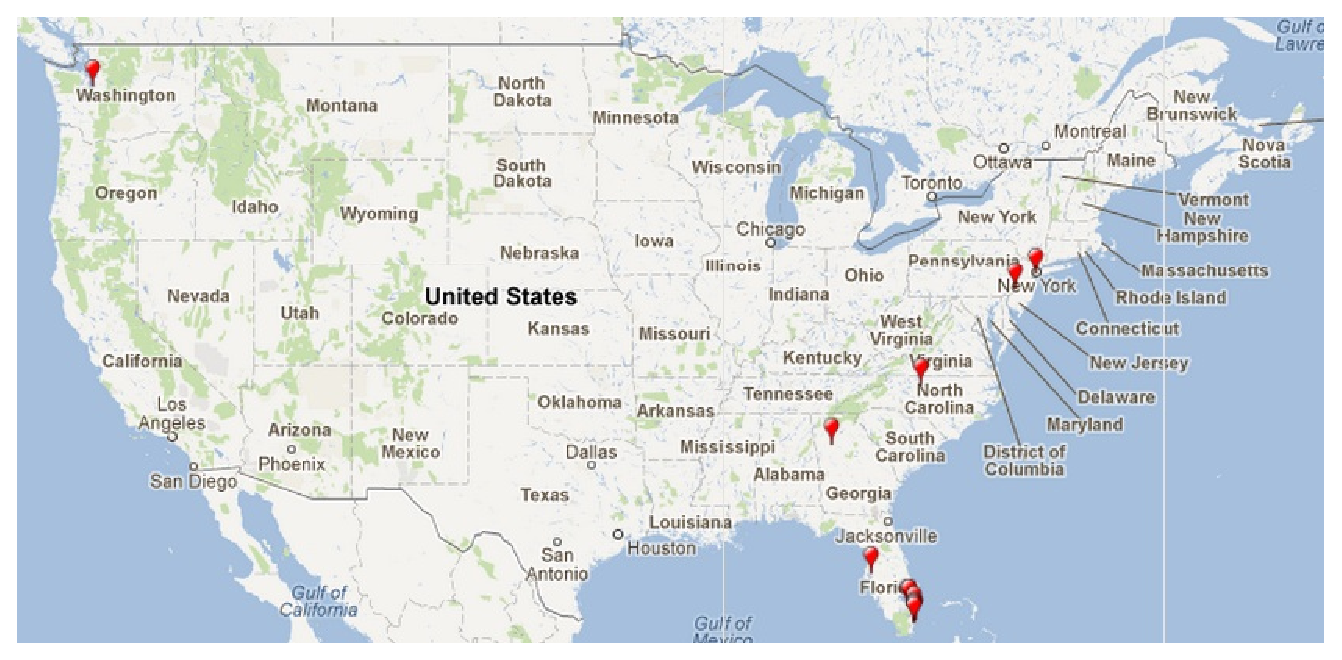
\includegraphics[width=0.6\columnwidth]{Figs/miami.eps}
\caption{
Tweet locations of an detected event.}
\label{fig:miami}
\end{figure}

To locate the impacted regions of the given anomaly,
we gather the authors of the collected tweets, which contains n-grams with high TF-IDF scores 
during the time frame.
Then we check the locations of the authors to get the impacted regions.
Figure~\ref{fig:miami} shows an example of the tweet locations for the anomaly occurred at Miami, 
FL. Although some users may tweet about network incidents from other locations,
as long as we see multiple tweets in a region, we can correctly locate the anomaly.  


%% =================================================================
\section{Conclusion}
\label{sec:conclusion}

We develop a systematic method to automatically detect anomalies in a
cellular network using the customer care call data. Our approach scales to a
large number of features in the data and is robust to 
noise. Using evaluation based on the call records collected from a
large cellular provider in US, we show that our method can
achieve 68\% recall and 86\% accuracy, much better than the existing
schemes.
Moreover, we show that social media can be used as a complementary source
to get higher confidence on the detected anomalies and to
summarize the user feedbacks to anomalies with text and location information.

%% =================================================================
